%%%%%%%% ICML 2026 EXAMPLE LATEX SUBMISSION FILE %%%%%%%%%%%%%%%%%

\documentclass{article}

% Recommended, but optional, packages for figures and better typesetting:
\usepackage{microtype}
\usepackage{graphicx}
\usepackage{subcaption}
\usepackage{booktabs} % for professional tables

% hyperref makes hyperlinks in the resulting PDF.
% If your build breaks (sometimes temporarily if a hyperlink spans a page)
% please comment out the following usepackage line and replace
% \usepackage{icml2026} with \usepackage[nohyperref]{icml2026} above.
\usepackage{hyperref}


% Attempt to make hyperref and algorithmic work together better:
\newcommand{\theHalgorithm}{\arabic{algorithm}}

% Use the following line for the initial blind version submitted for review:
%\usepackage{icml2026}

% For preprint, use
% \usepackage[preprint]{icml2026}

% If accepted, instead use the following line for the camera-ready submission:
 \usepackage[accepted]{icml2026}

\usepackage{amsmath}
\usepackage{amssymb}
\usepackage{mathtools}
\usepackage{amsthm}


% if you use cleveref..
\usepackage[capitalize,noabbrev]{cleveref}

%%%%%%%%%%%%%%%%%%%%%%%%%%%%%%%%
% THEOREMS
%%%%%%%%%%%%%%%%%%%%%%%%%%%%%%%%
\theoremstyle{plain}
\newtheorem{theorem}{Theorem}[section]
\newtheorem{proposition}[theorem]{Proposition}
\newtheorem{lemma}[theorem]{Lemma}
\newtheorem{corollary}[theorem]{Corollary}
\theoremstyle{definition}
\newtheorem{definition}[theorem]{Definition}
\newtheorem{assumption}[theorem]{Assumption}
\theoremstyle{remark}
\newtheorem{remark}[theorem]{Remark}

% Todonotes is useful during development; simply uncomment the next line
%    and comment out the line below the next line to turn off comments
%\usepackage[disable,textsize=tiny]{todonotes}
\usepackage[textsize=tiny]{todonotes}

% The \icmltitle you define below is probably too long as a header.
% Therefore, a short form for the running title is supplied here:
\icmltitlerunning{Seminar RLDMUU spring semester 2026}

\begin{document}

\twocolumn[
  \icmltitle{Principal-Agent Reinforcement Learning: \\
Orchestrating AI Agents with Contracts
}

  % It is OKAY to include author information, even for blind submissions: the
  % style file will automatically remove it for you unless you've provided
  % the [accepted] option to the icml2026 package.

  % List of affiliations: The first argument should be a (short) identifier you
  % will use later to specify author affiliations Academic affiliations
  % should list Department, University, City, Region, Country Industry
  % affiliations should list Company, City, Region, Country

  % You can specify symbols, otherwise they are numbered in order. Ideally, you
  % should not use this facility. Affiliations will be numbered in order of
  % appearance and this is the preferred way.
  \icmlsetsymbol{equal}{*}

  \begin{icmlauthorlist}
    \icmlauthor{Bustamante Isabelle}{Unifr}
    \icmlauthor{Meier Viola}{Unibe}
    \icmlauthor{Visetti Marta}{Unifr}

  \end{icmlauthorlist}

  \icmlaffiliation{Unifr}{Université de Fribourg, Switzerland}
  \icmlaffiliation{Unibe}{Universität Bern, Switzerland}


  \icmlcorrespondingauthor{Bustamante, Isabelle}{isabelle.bustamante@unifr.ch}
  \icmlcorrespondingauthor{Visetti, Marta}{marta.visetti@unifr.ch}

  % You may provide any keywords that you find helpful for describing your
  % paper; these are used to populate the "keywords" metadata in the PDF but
  % will not be shown in the document
  \icmlkeywords{Machine Learning, ICML}

  \vskip 0.3in
]

% this must go after the closing bracket ] following \twocolumn[ ...

% This command actually creates the footnote in the first column listing the
% affiliations and the copyright notice. The command takes one argument, which
% is text to display at the start of the footnote. The \icmlEqualContribution
% command is standard text for equal contribution. Remove it (just {}) if you
% do not need this facility.

% Use ONE of the following lines. DO NOT remove the command.
% If you have no special notice, KEEP empty braces:
\printAffiliationsAndNotice{}  % no special notice (required even if empty)
% Or, if applicable, use the standard equal contribution text:
% \printAffiliationsAndNotice{\icmlEqualContribution}

\begin{abstract}
We study the principal-agent reinforcement learning framework introduced by \citet{ivanov2024principal}, where a principal incentivizes a self-interested agent through outcome-based contracts in a sequential decision-making environment. We first reproduce the original meta-algorithmic setting under full knowledge of the MDP and then extend the framework using tabular Q-learning and Deep Q-learning, removing the assumption of known transition dynamics.\\
To evaluate the robustness of the learning dynamics, we conduct experiments on randomized principal-agent MDPs and compare the learned policies against oracle equilibrium solutions. Our results show that tabular Q-learning closely approximates the Subgame Perfect Equilibrium, achieving low empirical regret across environments. In contrast, Deep Q-learning exhibits substantially higher variance and instability, suggesting that the setup on which the test is conducted is not convenient with the method.\\
Finally, we investigate linear contracts as a restricted yet computationally simple contract class. Empirically, linear contracts recover nearly all of the principal’s utility while significantly reducing the complexity of contract optimization. Our findings highlight both the promise and the limitations of reinforcement learning approaches for dynamic contract design and incentive alignment in multi-agent systems.


\end{abstract}

\section*{Introduction}
Recent advances in artificial intelligence have led to the increasing deployment of autonomous AI agents in environments where decision-making, coordination, and incentive alignment play a central role. 
As these systems become more complex and autonomous, understanding how to design incentives that guide agent behaviour toward desired outcomes becomes an important research challenge.

A natural framework for studying such interactions is provided by principal-agent theory, a branch of economic contract theory that investigates how a principal can incentivize a self-interested agent through contracts and reward structures. Combined with reinforcement learning, this framework allows the study of adaptive agents operating in sequential decision-making environments.

In this work, we study the framework introduced by \cite{ivanov2024principal}, where a principal and an agent interact through contracts within a Markov Decision Process (MDP).

In the initial setting, both the principal and the agent have full knowledge of the underlying MDP, including the state space, transitions, outcomes, and reward structure. Under this assumption, the strategies of both parties are optimized iteratively until a Subgame Perfect Equilibrium (SPE) is reached.

Our goal is dual.
First, we reproduce part of the experimental setup and results presented in the original paper in order to better understand the proposed learning dynamics and incentive mechanisms. We first implement the proposed meta-algorithm in the fully observable setting, then extend it using Q-learning, and finally investigate a Deep Q-Learning approach where the underlying MDP is no longer assumed to be fully known. In this setting, policies are learned from sampled state transitions and rewards, which more closely reflects realistic reinforcement learning scenarios.

Second, we extend the framework by investigating the use of linear contracts and analyzing how different contract structures influence the learning behaviour of the agent.

The remainder of the paper is organized as follows.
Section~2 formalizes the principal-agent reinforcement learning framework and introduces the hidden-action MDP setting together with the notion of Subgame Perfect Equilibrium.
Section~3 presents the learning algorithms used in our implementation, including the meta-algorithm, tabular Q-learning, Deep Q-learning, and the extension based on linear contracts.
Section~4 reports the experimental results, including the replication of the original work, evaluations on randomized MDPs, and the analysis of linear contracts.
Finally, Section~5 concludes the paper and discusses limitations and directions for future work.

Unless stated otherwise, all algorithms, equations, and theoretical definitions follow~\cite{ivanov2024principal}.
% new structure Viola 
\section{Problem Formulation}

The principal-agent interaction is formulated as a Markov Decision Process (MDP). The environment is assumed to be fully known in the meta-algorithm setting, while in the Deep Q-Learning setting only sampled transitions and rewards are available.

\subsection{Hidden-Action Principal-Agent MDP}
\label{subsec:MDP}
The principal-agent MDP is defined as
\begin{equation}
M = (S, s_{0}, A, B, O, \mathcal{O}, \mathcal{R}, \mathcal{R^p}, \mathcal{T}, \gamma)
\end{equation}

Here, $S$ denotes the set of all states and $s_0 \in S$ the initial state. 
$A$ represents the set of possible actions available to the agent, while $B$ denotes the set of actions of the principal. The actions of the principal correspond to contracts $b(o)$ offered depending on observable outcomes.

The set of all possible outcomes is described by $O$. If the agent executes an action $a \in A$, an outcome $o \in O$ is generated stochastically. This is modeled by the outcome function
\[
\mathcal{O}: S \times A \xrightarrow{} \Delta(O).
\]

Higher effort by the agent can lead to better outcomes, although the results remain probabilistic rather than deterministic.

Based on the observed outcome and the current state, the environment transitions into the next state:
\[
s' \sim \mathcal{T}(s,o),
\]
where
\[
\mathcal{T}: S \times O \xrightarrow{} \Delta(S)
\]
defines the transition function.

The reward function of the agent is defined as
\[
\mathcal{R}(s,a,b,o) = r(s,a) + b(o),
\]
where $r(s,a)$ represents the intrinsic reward of the selected action and $b(o)$ the payment specified by the contract. The agent therefore aims to learn a strategy that maximizes its long-term reward.

The reward of the principal is defined by
\[
\mathcal{R}^{p}(s,b,o) = r^p(s,o) - b(o).
\]
The principal receives a reward depending on the resulting outcome, but simultaneously has to pay the contractual compensation to the agent.

The term Hidden-Action refers to the fact that the actual action chosen by the agent is not directly observable to the principal. The principal only observes the resulting outcome $o \in O$, which depends probabilistically on the selected action. Consequently, contracts are based on observable outcomes rather than directly on the agent's actions. As a result, the reward of the principal only depends indirectly on the agent's action and is modeled solely through the outcome.

The parameter $\gamma \in [0,1]$ denotes the discount factor, which determines the importance of future rewards compared to immediate rewards.

\paragraph{Interaction Procedure}
The interaction is modeled as a stochastic game in which both players aim to maximize their long-term rewards.

In timestep $t$, the principal observes the current state $s_t$ and offers a contract $b_t$ according to its policy
\[
\rho: S \xrightarrow{} \Delta(B).
\]

The agent then observes the pair $(s_t, b_t)$ and selects an action according to its policy
\[
\pi: S \times B \xrightarrow{} \Delta(A).
\]

Based on the selected action, an outcome $o \in O$ is stochastically sampled according to the distribution of the results. The MDP then transitions to the next state $s_{t+1}$.

This interaction is repeated sequentially, while both parties attempt to maximize their respective value functions over time.

The solution of the stochastic game is described in Section~\ref{subsec:meta_algorithm}.

\subsection{Incentive Compatibility and Individual Rationality}
Two standard constraints from contract theory govern the design of feasible contracts in this setting.

\textbf{Incentive Compatibility (IC)} requires that the contract makes the agent willing to choose the action desired by the principal. Formally, for a recommended action $a^p \in A$, the contract $b$ must satisfy
\[
\begin{aligned}
&\mathbb{E}_{o \sim \mathcal{O}(s,a^p)}[r(s,a^p) + b(o)] \\
&\quad \geq \mathbb{E}_{o \sim \mathcal{O}(s,a)}[r(s,a) + b(o)] \quad \forall\, a \neq a^p,
\end{aligned}
\]
ensuring that the agent's expected utility under $a^p$ is at least as large as under any deviation.

\textbf{Individual Rationality (IR)} requires that the agent's expected utility under the contract is non-negative, i.e., that participation is preferable to opting out:
\[
\mathbb{E}_{o \sim \mathcal{O}(s,a^p)}[r(s,a^p) + b(o)] \geq 0.
\]

Together, IC and IR ensure that the contract is both self-enforcing and acceptable to the agent. In the principal-agent MDP setting, these constraints are imposed at every state $s \in S$ and are embedded in the linear program solved by the principal at each step of the learning process.
\subsection{Subgame Perfect Equilibrium}

The interaction between the principal and the agent can be interpreted as a sequential stochastic game.
At each timestep, the principal first proposes a contract, after which the agent selects an action in response to the offered incentives.
Since decisions are made repeatedly over time and future states depend on previous actions and outcomes, the setting naturally fits the framework of dynamic game theory.

In such sequential settings, a standard Nash Equilibrium is generally insufficient, since it only guarantees that no player has an incentive to deviate globally from its strategy.
Instead, the appropriate solution concept is the Subgame Perfect Equilibrium (SPE), which requires that strategies remain optimal in every subtree of the game.

Formally, in our setting, an SPE is a strategy profile $(\rho^*, \pi^*)$ such that:
\begin{itemize}
    \item the principal policy $\rho^*$ maximizes the expected long-term utility of the principal,
    \item the agent policy $\pi^*$ maximizes the expected long-term utility of the agent given the contracts offered by the principal,
    \item neither player benefits from deviating at any reachable state of the stochastic game.
\end{itemize}

In the meta-algorithm, the principal and the agent iteratively update their strategies until convergence toward an SPE is achieved.
The principal optimizes the offered contracts assuming a rational best response from the agent, while the agent optimizes its policy under the current contractual incentives.

In the Q-learning extension, the same equilibrium structure is approximated through sampled interactions with the environment rather than complete knowledge of the MDP dynamics.
Instead of computing exact optimal responses, both players learn their policies from observed rewards and transitions.
Consequently, the learned policies approximate an SPE empirically through repeated interactions and value-function updates.

\section{Algorithms}
\textbf{Environment}\\
\label{sec:simple}
In a first setting, the implemented algorithms perform over a simple initialization of the hidden-action principal-agent MDP as presented in the paper \cite{ivanov2024principal}.The stochastic game is modeled as an infinite-horizon discounted interaction. 
\begin{figure} [H]
    \centering
    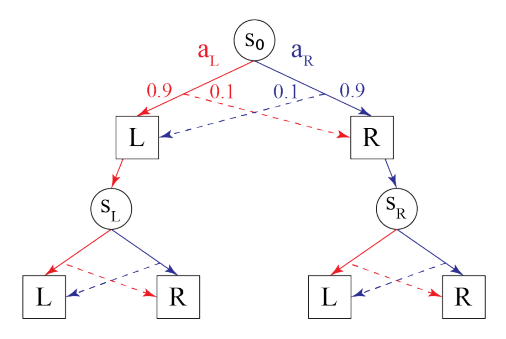
\includegraphics[width=0.8\linewidth]{figures/simple_MDP.png}
    \caption{Example of a principal-agent MDP, as in paper \cite{ivanov2024principal}}
    \label{fig:placeholder}
\end{figure}
The MDP has three states $S=\{s_0,s_L,s_R\}$, at each the agent can chose between two actions $A=\{a_L,a_R\}$ who can lead to a specific outcome $O=\{L,R\}$. The distribution of outcome L taking action $a_L$ is of 0.9, while taking action $a_R$ it is of 0.1; the distribution of outcome R is of 0.9 when taking action $a_R$ and of 0.1 when taking action $a_L$.\\ 

Agent and principal have different rewards for a certain outcome or action at state $s \in S$. At $(s,L)$ the principal has reward $14\over9$, while at $(s,R)$ his reward is $0$. The agent's intrinsic reward is $r(s,a_L) = -\frac{4}{5}$, making action $a_L$ costly, while $r(s,a_R) = 0$


\subsection{Meta-algorithm}
\label{subsec:meta_algorithm}
The first implemented approach follows the meta-algorithm proposed in \cite{ivanov2024principal}.
The method performs an iterative bilevel optimization over the policies of both the principal and the agent within the principal-agent MDP introduced in Section~\ref{subsec:MDP}.


In this setting, both actors are assumed to have complete knowledge of the environment, including the transition dynamics, outcome distributions, and reward functions. Under this assumption, optimal policies can be computed exactly using dynamic programming methods. In our implementation, both the inner and outer optimization problems are solved using value iteration.


The algorithm alternates between two optimization steps.
In the inner optimization, the agent computes a best-response policy maximizing its expected long-term utility under the currently offered contracts.
In the outer optimization, the principal computes the contract that maximizes its own expected utility given the agent's current best-response policy.


This iterative process continues until the policies of both players stabilize. The resulting strategy profile approximates a Subgame Perfect Equilibrium (SPE), in which neither the principal nor the agent has an incentive to deviate at any reachable state of the stochastic game. 

\subsection{Q-Learning}
\label{subsec:Qlearning}
Starting from the setting defined in the meta-algorithm, we apply reinforcement learning to approximate the equilibrium through repeated interactions with the environment. The underlying MDP remains the same as the one described in Section~\ref{subsec:MDP}, but both the inner and outer optimization problems are now solved using Q-learning. \\
The framework consists of two independent learners:
the agent learns which action to execute under a given contract, while the principal learns which action to incentivize and which contract induces the desired behaviour at minimal cost.
\paragraph{Agent Q-Learning}

The agent observes the current state $s$ together with the contract $b$ offered by the principal and learns a policy
\[
\pi : S \times B \rightarrow \Delta(A).
\]
Following \cite{ivanov2024principal}, the agent uses a truncated Q-function:
\[
Q^{*}((s,b),a) = \mathbb{E}[b(o)] + \bar{Q}(s,a),
\]
where $\bar{Q}(s,a)$ captures the long-term value of executing action $a$ in state $s$, independently of the current contract.
The agent updates $\bar{Q}(s,a)$ using the standard Q-learning update rule:
\[
\begin{aligned}
\bar{Q}(s,a)
\leftarrow\;&
\bar{Q}(s,a)
+
\alpha
\Big[
r(s,a)
+
\gamma \max_{a'} Q^{*}((s',b'),a')
\\
&-
\bar{Q}(s,a)
\Big].
\end{aligned}
\]
Action selection is performed using an $\epsilon$-greedy exploration strategy.
With probability $\epsilon$, a random action is selected, while otherwise the agent chooses the action with maximal estimated utility.

\paragraph{Principal Q-Learning}

The principal simultaneously learns which action should be induced in each state.
Instead of directly learning contracts, the principal maintains a Q-table
\[
Q^{p}(s,a^{p}),
\]
which estimates the expected long-term utility obtained when attempting to induce action $a^{p}$ in state $s$.

At every timestep, the principal first selects a target action using an $\epsilon$-greedy policy over its Q-values.
Given the selected target action, the principal then computes the cheapest feasible contract that incentivizes the agent to choose this action.

The optimal contract is obtained by solving a linear program:
\[
\max_{b \in B}
\mathbb{E}_{o \sim \mathcal{O}(s,a^{p})}[-b(o)],
\]
subject to incentive compatibility constraints ensuring that the agent prefers the intended action over all alternatives.

After observing the resulting outcome and transition, the principal updates its Q-values according to
\[
\begin{aligned}
Q^{p}(s,a^{p})
\leftarrow\;&
Q^{p}(s,a^{p})
+
\alpha
\Big[
r^{p}(s,o)-b(o)
\\
&+
\gamma \max_{a'} Q^{p}(s',a')
-
Q^{p}(s,a^{p})
\Big].
\end{aligned}
\]

Through repeated interactions, both learners adapt simultaneously:
the agent improves its behavioural policy under contracts, while the principal learns how to design contracts that maximize its own long-term reward.

\subsection{Deep Q-Learning}
Building on the tabular Q-learning framework, we extended both learners to function approximation using Deep Q-Networks, described in Algorithm~\ref{alg:deep-q}. Following~\cite{ivanov2024principal}, this approach was introduced to 
empirically validate the convergence of the meta-algorithm towards the SPE. 
We used the underlying MDP unchanged to allow a direct comparison with the analytical SPE solution as well as the results from tabular Q-learning. In section~\ref{subsec:replication} we compare all algorithms on different MDP's with random outcome distribution. 
The Q-tables are replaced by neural networks parametrized by $\theta$ (principal) and $\phi$ (agent). 

\paragraph{Agent Deep Q-Learning}
The agent's network $\bar{Q}^{\phi}(s,a)$ approximates the truncated 
Q-values, so the expected long-term utility excluding the immediate payment, as described in the previous section.  The full Q-value is then recovered as
\[
Q^{*}((s,b),a) = \mathbb{E}_{o \sim \mathcal{O}(s,a)}[b(o)] 
+ \bar{Q}^{\phi}(s,a).
\]
To ensure that $\phi$ learns the truncated rather than the standard Q-function, the target $y^a$ is computed using the contract $b^*$ of the next state $s'$:
\[
y^{a}(s,a^{p}) = r^{a} + \gamma(1-d)
\Bigl(
\mathbb{E}_{o'}[b^{*}(s',a^{p'},o')]
+\bar{Q}^{\phi'}(s',a^{p'})
\Bigr),
\]
where $o' \sim \mathcal{O}(s',a^{p'})$.

\paragraph{Principal Deep Q-Learning}
The principal's network $q^{\theta}(s,a^p)$ estimates the expected long-term utility of incentivizing action $a^p$ in state $s$. Given the selected target action, the optimal contract $b^*(s,a^p)$ is computed 
by solving the LP.
The target is then
\[
y^{p}(s,a^{p}) = r^{p} - b^{*}(s,a^{p},o)
+ \gamma(1-d)\,q^{\theta'}(s',a^{p'})
\]

\paragraph{Training Setup}
Both networks consist of two hidden layers with 256 neurons and ReLU activations, and are trained simultaneously from a replay buffer of size 20\,000 with mini-batches of 128, following the suggestions of \cite{ivanov2024principal}.
Target networks are updated every 100 iterations. The learning rate and exploration rate $\epsilon$ are annealed from $0.001$ to $0.0001$ and from $1$ to $0$, respectively.

\subsection{Linear Contracts}
\label{subsec:linear_contracts}

A linear contract is parameterised by a single sharing ratio $\alpha \in [0,1]$: the agent receives a fixed fraction $\alpha$ of the principal’s realised reward, and the principal retains $(1-\alpha)$. Formally, $b(o) = \alpha \cdot r^p(s, o)$. This reduces the entire contract to a single parameter, rather than a separate payment per outcome.

\paragraph{Incentive Compatibility}
The contract is incentive compatible for the recommended action $a^p$ if:
\[
\begin{aligned}
  &\alpha \cdot \mathbb{E}_{o \sim \mathcal{O}(s,a^p)}[r^p(s,o)] + \bar{Q}(s,a^p) \\
  &\quad \geq\; \alpha \cdot \mathbb{E}_{o \sim \mathcal{O}(s,a)}[r^p(s,o)] + \bar{Q}(s,a)
  \quad \forall\, a \neq a^p,
\end{aligned}
\]
where $\bar{Q}(s,a)$ is the agent’s Q-estimate of long-term payoff net of payments. Any candidate $\alpha$ that violates this constraint is discarded.

\paragraph{Principal’s Optimization}
The principal performs a grid search over 100 evenly spaced values of $\alpha$ and selects the incentive-compatible candidate that maximises its expected net revenue:
\[
  \alpha^* = \arg\max_{\alpha \;\text{IC-feasible}} \;(1 - \alpha) \cdot \mathbb{E}_{o \sim \mathcal{O}(s,a^p)}[r^p(s,o)].
\]
If no feasible $\alpha$ exists, the principal offers the null contract $b \equiv 0$.

\paragraph{Approximation Bound}
\citet{dutting2024survey} show that the worst-case approximation ratio $\rho$ between the optimal LP contract and the best linear contract is at most $n$, the number of \emph{actions}. With $n = 2$ actions, $\rho \leq 2$. In binary-outcome settings where one action has reward 0, a linear contract is in fact optimal and $\rho = 1$; more generally, as the reward for one action approaches zero, $\rho \to 1$.

\section{Results and Discussion}
\subsection{Replication of Original Results}
We first reproduce the experimental setting proposed in \citet{ivanov2024principal} in order to validate our implementation of the principal-agent framework and verify the convergence behaviour of the proposed algorithms.\\
The experiments are conducted on the same hidden-action principal-agent MDP described in Section~\ref{sec:simple}. In this setting, the principal iteratively optimizes contracts while the agent learns a best-response policy. Following the original paper, we evaluate whether the learning dynamics converge toward a Subgame Perfect Equilibrium (SPE), and compare the learned utilities against the oracle solution obtained through value iteration.\\
Our implementation successfully reproduces the main qualitative findings reported in the original work. In the fully observable setting, the meta-algorithm consistently converges toward stable policies for both the principal and the agent. The resulting utilities closely match the analytical SPE solution, confirming the correctness of the bilevel optimization procedure.\\
Similarly, the tabular Q-learning implementation empirically converges toward the oracle solution across most runs. The learned contracts successfully incentivize the desired actions while maintaining low regret with respect to the equilibrium policy. These results support the claim of \citet{ivanov2024principal} that reinforcement learning can recover approximately incentive-compatible contracts through repeated interaction.\\
In contrast, the Deep Q-learning implementation exhibits substantially less stable behaviour. While some runs converge toward near-optimal policies, others become trapped in suboptimal equilibria or exhibit oscillatory learning dynamics. Compared to the original paper, our implementation shows higher empirical variance and lower average utility for the principal. We hypothesize that this discrepancy is partly caused by the sensitivity of Deep Q-learning to hyperparameter choices and initialization, as well as the non-stationarity introduced by the contract optimization process itself.\\
Overall, the experiments confirm the reproducibility of the original framework in the tabular setting while also highlighting the practical challenges of extending the approach to deep function approximation methods.

\subsection{Performance over Randomized MDPs}
\label{subsec:replication}
To further evaluate our implementation, we extend the experimental setting to 100 randomly generated MDPs. Each MDP shares the same structure as the one presented in Section~\ref{sec:simple}, while the transition probabilities are randomized independently for every experiment instance by sampling from a Dirichlet distribution for each state-action pair. For each instance, we extract the induced policies, the principal's expected utility, and the corresponding regret with respect to the oracle solution.



The \textbf{Q-learning experiments }are run with the following hyperparameters. We consider $N_{\mathrm{MDP}} = 100$ independent MDP instances to average performance across environments and reduce variance. The discount factor is set to $\gamma = 1$, implying no temporal discounting and equal weighting of future and immediate rewards. Each experiment consists of $N_{\mathrm{META}} = 20$ meta-iterations, where each iteration corresponds to a full round of training the principal-agent interaction. Within each meta-iteration, the learning process is carried out over $N_{\mathrm{EPISODES}} = 5000$ episodes. The learning rate for Q-updates is set to $\alpha = 0.1$, and an $\epsilon$-greedy exploration strategy is used with $\epsilon = 0.1$ to balance exploration and exploitation for both the principal and the agent.\\
In the conditions of the experiment, Q-learning is performing well, the SPE utility of the principal matches almost always the oracle one, the mean of the Q-Learning principal's utility has a negative difference of less than 0.03 compared to the one he achieves in the oracle run and the mean regret found is of the $2.75\%$, as one can compare with Table~\ref{tab:utility_regret} and Appendix~\ref{app:qlearn100}.
\begin{table}[H]
\centering
\begin{tabular}{lcc}
\hline
\textbf{Metric} & \textbf{Mean} & \textbf{Std} \\
\hline
Oracle utility & 0.8033 & 0.2840 \\
QL utility    & 0.7757 & 0.2938 \\
Regret        & 0.0275 & 0.1424 \\
Regret \%     & 2.75\% & -- \\
\hline
\end{tabular}
\caption{Summary statistics of utility and regret metrics for Q-learning evaluation}
\label{tab:utility_regret}
\end{table}

\begin{figure}[H]
    \centering
    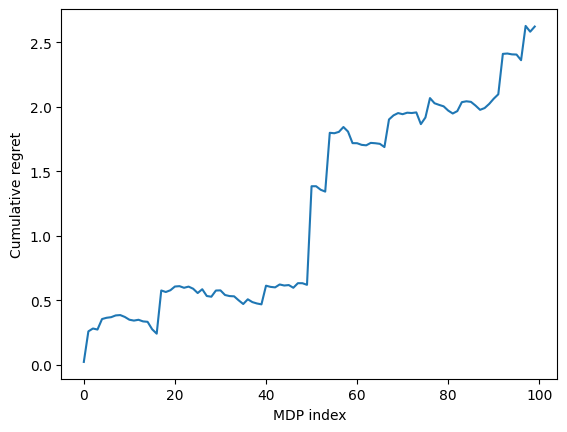
\includegraphics[width=0.8\linewidth]{figures/cumulative_regret_100_run_qlearn.png}
    \caption{Cumulative regret for Q-learning experiment}
    \label{fig:cumulativeqlearn}
\end{figure}

To further investigate \textbf{Q-learning, we repeat the pipeline while allowing the agent’s learned Q-function to be transferred across consecutive MDP instances}. The resulting performance is reported in Appendix~\ref{app:qlearnknow}. Interestingly, this setup can lead to slightly negative regret in some cases. In general the SPE is almost reached, hence both the principal and agent are in equilibrium, these cases of negative regret, registered here for the principal, are probably due to some delta between the oracle's SPE and the learned one. This induces that one party might have higher utility, while the other has opposite consequences. When consecutive MDPs exhibit similar structural patterns, the learning procedure may benefit from implicit transfer, yielding a marginal advantage over the fully re-initialized oracle comparison. This is reflected in a lower general regret in comparison with the previous Q-learning experiment and is quite noticeable in the patterns generated over the cumulative regret, where instead of finding some plateaus, we have some descending trends.

\begin{table}[h]
\centering
\begin{tabular}{lcc}
\hline
\textbf{Metric} & \textbf{Mean} & \textbf{Std} \\
\hline
Oracle utility & 0.8309 & 0.2688 \\
QL utility    & 0.8155 & 0.2911 \\
Regret        & 0.0154 & 0.0912 \\
Regret \%     & 2.08\% & -- \\
\hline
\end{tabular}
\caption{Summary statistics of utility and regret metrics for Q-learning with transmission of knowledge evaluation}
\label{tab:knows}
\end{table}

\begin{figure} [H]
    \centering
    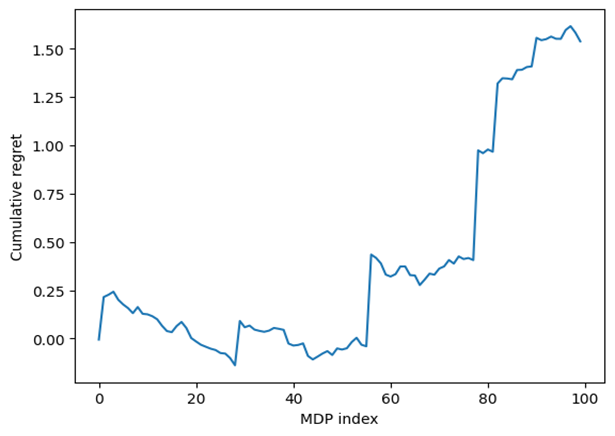
\includegraphics[width=0.75\linewidth]{figures/cumulative_knowl.png}
    \caption{Cumulative regret for Q-learning with transfer of knowledge experiment}
    \label{fig:cumulativeknowledge}
\end{figure}

The \textbf{Deep Q-learning experiments} follow the same randomized MDP setting, with $N_{MDP}=100, \gamma = 1$, and training performed over 20000 iterations with a network update every 100 iterations through experience replay. As shown in Table~\ref{tab:dqtable}, the mean regret reaches 42.44\%, a dramatic increase relative to the tabular setting. We hypothesize that the origin of this degradation might primarily be due to the interaction between function approximation and the bilevel structure of the problem: small estimation errors in early training propagate through the contract optimization step, destabilizing incentives and occasionally causing policy collapse. Notably, despite the higher regret, the cumulative regret curves exhibit more pronounced plateau regions than in the tabular case, suggesting that Deep Q-learning converges prematurely to locally stable but suboptimal incentive structures rather than continuing to make corrective updates over time.
\begin{table}[h]
\centering
\begin{tabular}{lcc}
\hline
\textbf{Metric} & \textbf{Mean} & \textbf{Std} \\
\hline
Oracle utility & 0.8110 & 0.2656 \\
QL utility    & 0.4642 & 0.7051 \\
Regret        & 0.3468 & 0.7059 \\
Regret \%     & 42.44\% & -- \\
\hline
\end{tabular}
\caption{Summary statistics of utility and regret metrics for deep Q-learning evaluation}
\label{tab:dqtable}
\end{table}

\begin{figure} [H]
    \centering
    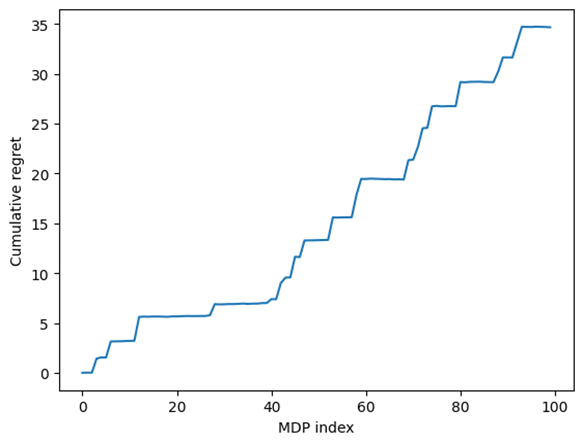
\includegraphics[width=0.75\linewidth]{figures/cumulative_regr_ql.png}
    \caption{Cumulative regret for deep Q-learning experiment}
    \label{fig:regretql}
\end{figure}


\subsection{Application of Linear Contracts}
\label{subsec:results_linear}

We evaluate both contract designs on 30 randomly generated MDPs. As noted in Section~\ref{subsec:linear_contracts}, the original fixed MDP has $r^p(s,R) = 0$, which by Proposition 3.9 \citep{dutting2024survey} makes a linear contract already optimal. We therefore randomise all MDP parameters while keeping the same structure (2 actions, 2 outcomes, 1 non-terminal state): transition probabilities are Dirichlet-sampled, action costs are drawn uniformly from $[0,1]$, and principal rewards from $[0,2]$. For each instance, the Q-learning agent is trained once; both contract methods are then evaluated from the same learned Q-values, with expected utilities computed analytically from the known transition probabilities, so that any observed difference in utility reflects the contract structure rather than training variance. The approximation ratio $\rho = U_{\mathrm{LP}} / U_{\mathrm{Linear}}$ shows the cost of restricting to linear contracts. The bound $\rho \leq 2$ from Section~\ref{subsec:linear_contracts} was established for the static model; we verify whether this applies to the Q-learning setting.

\begin{table}[ht]
  \caption{Principal utility and approximation ratio $\rho$ across 30 random MDPs.}
  \label{tab:linear_results}
  \begin{center}
    \begin{small}
      \begin{sc}
        \begin{tabular}{lcc}
          \toprule
           & Mean & Std \\
          \midrule
          $U_{\mathrm{LP}}$ (unrestricted) & 1.1256 & 0.4248 \\
          $U_{\mathrm{Linear}}$             & 1.1029 & 0.4116 \\
          Approximation ratio $\rho$        & 1.0198 & 0.0929 \\
          \midrule
          Theoretical bound ($n=2$ actions) & \multicolumn{2}{c}{$\rho \leq 2$} \\
          \bottomrule
        \end{tabular}
      \end{sc}
    \end{small}
  \end{center}
  \vskip -0.1in
\end{table}

The mean approximation ratio of $\rho = 1.02$ (std $= 0.09$) indicates that linear contracts recover approximately $98\%$ of the principal’s utility on average, far below the theoretical worst-case bound of $2$. As expected from \citet{dutting2024survey}, in binary-outcome settings where one action has reward 0 the linear contract is already optimal ($\rho = 1$), and our randomised environments are close enough to this structure that the empirical ratios stay near $1$.




\section*{Conclusion}
In this work, we reproduced and extended the principal-agent reinforcement learning framework by \citet{ivanov2024principal}. We first implemented the original meta-algorithm under full knowledge of the environment and subsequently investigated tabular and deep reinforcement learning approaches in settings where the MDP dynamics are not explicitly known.

Our experiments show that tabular Q-learning successfully approximates the oracle Subgame Perfect Equilibrium across a large set of randomized environments, achieving consistently low empirical regret. These results suggest that incentive-compatible contracts can be learned effectively through repeated interaction even without explicit knowledge of the environment dynamics. Furthermore, we observed that transferring learned Q-values across related MDPs can further improve performance, indicating that incentive structures may generalize across similar environments.

In contrast, Deep Q-learning exhibited significantly higher instability and regret. We argue that this degradation originates from the interaction between function approximation and the bilevel optimization structure of the principal-agent problem. Because the principal continuously modifies the reward landscape through contracts, the agent faces a highly non-stationary learning objective, which may amplify approximation errors and lead to premature convergence toward suboptimal equilibria.

Finally, we investigated linear contracts, which restrict the contract space to a single sharing parameter. In our experiments, they recovered nearly all of the utility achieved by unrestricted LP-based contracts. The results suggest that, at least in low-dimensional settings, the gain from using more expressive contracts is small, and the simplicity of linear contracts may be worth the minor loss in principal utility.

Overall, our findings support the potential of combining contract theory and reinforcement learning for AI alignment and multi-agent coordination problems, while also highlighting important limitations of current deep reinforcement learning methods in strategic bilevel settings. Future work could investigate more stable deep RL algorithms, partially observable environments, richer contract spaces, and transfer learning mechanisms for incentive design.
Furthermore, in the present setting the outcome distribution function $\mathcal{O}(s,a)$ is assumed to be known, which may not hold in realistic scenarios. An avenue for future work is therefore to approximate this function through an additional neural network, as suggested in the paper, moving towards settings with less restrictive assumptions on environment knowledge.



% old structure: 
% \section{Related Work}
% \subsection{Contract Theory}
% \cite{dutting2024survey}
% \subsection{Multi-Agent Reinforcement Learning}
% % \subsection{Principal-Agent RL}

% \section{Game-Theoretic Foundations}
% \subsection{Principal-Agent Games}
% \subsection{Subgame Perfect Equilibrium}

% \section{Problem Formulation}
% \subsection{Principal}
% \subsection{Agent}
% \subsection{Contract Space}
% \subsection{MDP Formulation}
% \subsection{Reward Structure}
% \subsection{Equilibrium Concept (SPE)}


% \section{Implementation}

% \section{Results}
% \subsection{Replication of Original Results}
% \subsection{Application of linear contracts}

% \section{Discussion}

% \section*{Conclusion}



% In the unusual situation where you want a paper to appear in the
% references without citing it in the main text, use \nocite
\nocite{langley00}

\bibliography{example_paper}
\bibliographystyle{icml2026}

%%%%%%%%%%%%%%%%%%%%%%%%%%%%%%%%%%%%%%%%%%%%%%%%%%%%%%%%%%%%%%%%%%%%%%%%%%%%%%%
%%%%%%%%%%%%%%%%%%%%%%%%%%%%%%%%%%%%%%%%%%%%%%%%%%%%%%%%%%%%%%%%%%%%%%%%%%%%%%%
% APPENDIX
%%%%%%%%%%%%%%%%%%%%%%%%%%%%%%%%%%%%%%%%%%%%%%%%%%%%%%%%%%%%%%%%%%%%%%%%%%%%%%%
%%%%%%%%%%%%%%%%%%%%%%%%%%%%%%%%%%%%%%%%%%%%%%%%%%%%%%%%%%%%%%%%%%%%%%%%%%%%%%%
\newpage
\appendix
\onecolumn
\section{Appendix}
\subsection{Source code}
The source code for the implementation presented in this report is available on GitHub:
\href{https://github.com/martavise/Seminar_RLDMUU_AI_agents_contracts}{martavise/Seminar\_RLDMUU\_AI\_agents\_contracts}.
\subsection{Meta-algorithm}
\begin{algorithm}
  \caption{Meta-algorithm for finding SPE}
  \label{alg:spe-meta}
  \begin{algorithmic}
    \STATE \textbf{Require:} principal policy $\rho$, agent policy $\pi$
    \STATE Initialize the principal’s policy $\rho$ arbitrarily (e.g., $\forall s \in S: \rho(s) = 0$)
    
    \WHILE{$\rho$ not converged}
      \STATE Solve the agent’s MDP: find $\pi := \pi^{*}(\rho)$
      \STATE Solve the principal’s MDP: find $\rho := \rho^{*}(\pi)$
    \ENDWHILE
    
    \STATE \textbf{return} $(\rho, \pi)$
  \end{algorithmic}
\end{algorithm}


\subsection{Deep Q-learning}
\begin{algorithm}[H]
  \caption{Deep Q-learning}
  \label{alg:deep-q}
  \begin{algorithmic}
    \STATE \textbf{Require:} principal's Q-network $\theta$, agent's Q-network 
    $\phi$, target networks $\theta'$ and $\phi'$, replay buffer $RB$
    \STATE Initialize buffer $RB$ with random transitions, networks $\theta$ 
    and $\phi$ with random parameters
    \FOR{number of updates}
      \FOR{number of interactions per update}
        \STATE Select an action to recommend $a^p$ with $q^{\theta}(s,a)$ 
        via $\epsilon$-greedy
        \STATE Sample $o \sim \mathcal{O}(s,a)$,\; $r^a = r(s,a)$,\; 
        $r^p = r^p(s,o)$,\; transition the MDP to $s' \sim \mathcal{T}(s,o)$
        \STATE Add the transition $(s,\,a^p,\,r^a,\,r^p,\,o,\,d,\,s')$ 
        to the buffer $RB$
        \STATE If $d=1$, reset the MDP
      \ENDFOR
      \STATE Sample a mini-batch of transitions $mb \sim RB$
      \FOR{$(s,\,a^p,\,r^a,\,r^p,\,o,\,d,\,s') \in mb$}
        \STATE $a^{p'} = \arg\max_{a'}\, q^{\theta}(s',a')$
        \STATE Find optimal contracts $b^*(s,a^p)$ and $b^*(s',a^{p'})$ 
        by solving LP~(3)
        \STATE $y^p(s,a^p) = r^p - b^*(s,a^p,o) 
        + \gamma(1-d)\,q^{\theta'}(s',a^{p'})$
        \STATE $y^a(s,a^p) = r^a + \gamma(1-d)
        \Bigl(\mathbb{E}_{o' \sim \mathcal{O}(s',a^{p'})}\bigl[b^*(s',a^{p'},o')\bigr] 
        + \bar{Q}^{\phi'}(s',a^{p'})\Bigr)$
      \ENDFOR
      \STATE Minimize $L(\theta) = 
      \displaystyle\sum_{mb}\!\bigl(q^{\theta}(s,a^p)-y^p(s,a^p)\bigr)^2$
      \STATE Minimize $L(\phi) = 
      \displaystyle\sum_{mb}\!\bigl(\bar{Q}^{\phi}(s,a^p)-y^a(s,a^p)\bigr)^2$
    \ENDFOR
  \end{algorithmic}
\end{algorithm}
Algorithm from \cite{ivanov2024principal}, page 35.

\subsection{Results of evaluation of Q-Learning over 100 MDPs}
\label{app:qlearn100}
\begin{figure} [H]
    \centering
    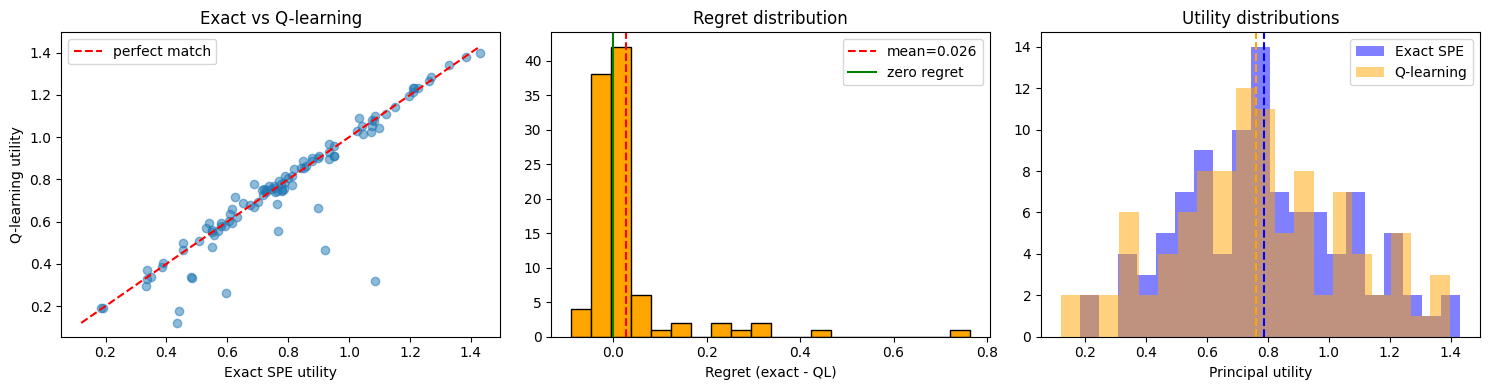
\includegraphics[width=1\linewidth]{figures/result_100_run_meta_qlearn.png}
    \caption{SPE comparison, principal utility and regret comparison between oracle and Q-learning}
    \label{fig:graphs100qlearn}
\end{figure}


\subsection{Results of evaluation of Q-Learning with transmission of knowledge}
\label{app:qlearnknow}
\begin{figure} [H]
    \centering
    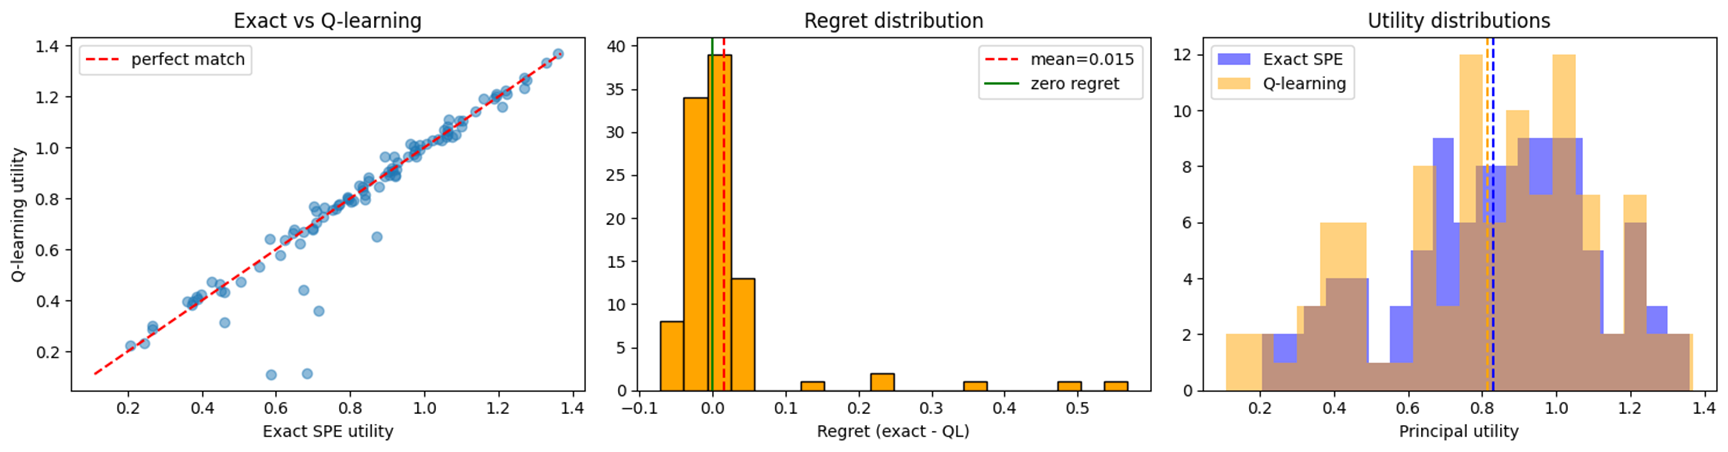
\includegraphics[width=1\linewidth]{figures/qlearning_policytransmitted.png}
    \caption{SPE comparison, principal utility and regret comparison between oracle and Q-learning with transmission of knowledge}
    \label{fig:graphs100knowledge}
\end{figure}

\subsection{Results of evaluation of deep Q-learning over 100 MDPs}
\begin{figure} [H]
    \centering
    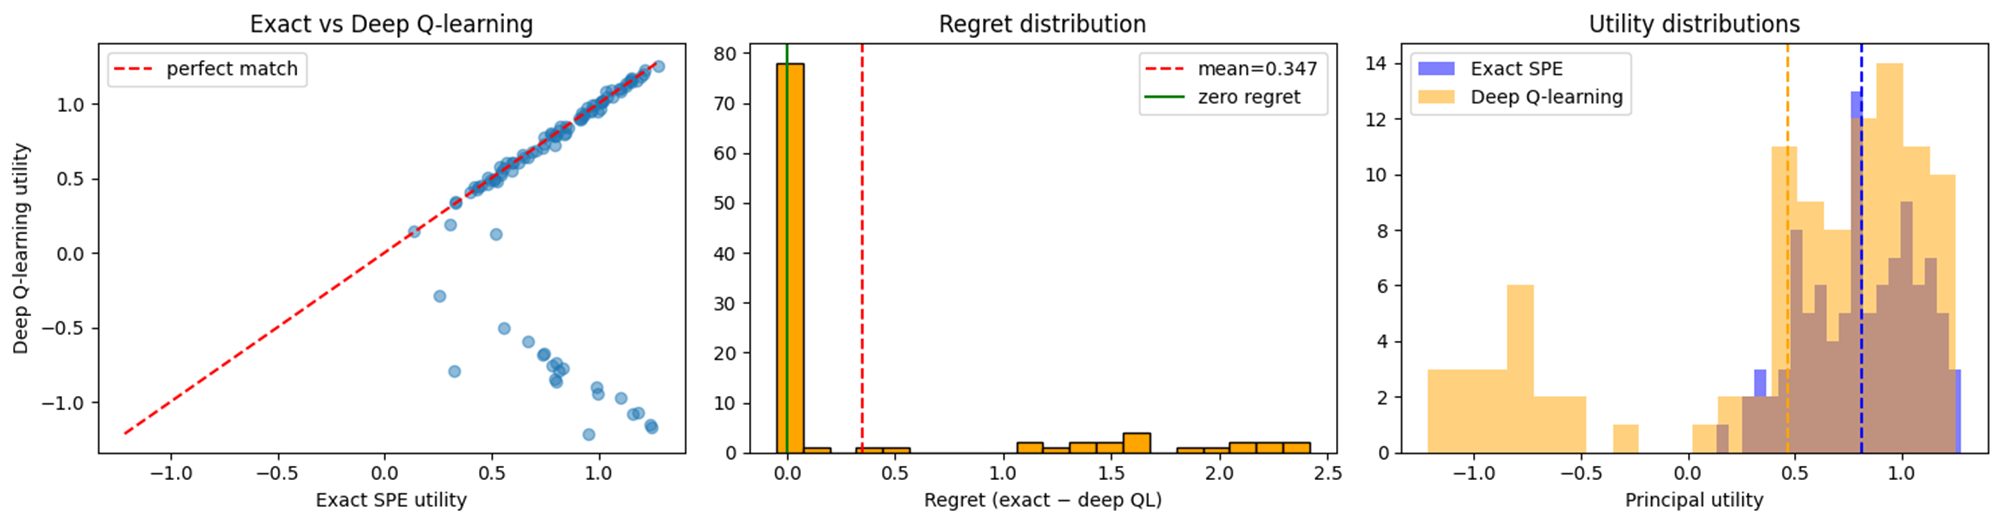
\includegraphics[width=1\linewidth]{figures/deepq_vsoracle.png}
    \caption{SPE comparison, principal utility and regret comparison between oracle and deep Q-learning}
    \label{fig:graphsdeepq}
\end{figure}
% ATM it's just a buch of examples
% You can have as much text here as you want. The main body must be at most $8$
% pages long.

% The $\mathtt{\backslash onecolumn}$ command above can be kept in place if you
% prefer a one-column appendix, or can be removed if you prefer a two-column
% appendix.  Apart from this possible change, the style (font size, spacing,
% margins, page numbering, etc.) should be kept the same as the main body.

\subsection{Use of external aid}
As a code base for the RL algorithms, the lab materials from the RL lecture FS2026 at the University of Neuchâtel were used and adapted to the present setup.
Claude (claude-sonnet-4-6) was used to assist in writing the linear contracts section, for general code refactoring and corrections, and to verify that the implementation of the functions corresponded to the intended behaviour described in the paper. ChatGPT was used to help rephrase some paragraphs and check general grammar.





%%%%%%%%%%%%%%%%%%%%%%%%%%%%%%%%%%%%%%%%%%%%%%%%%%%%%%%%%%%%%%%%%%%%%%%%%%%%%%%
%%%%%%%%%%%%%%%%%%%%%%%%%%%%%%%%%%%%%%%%%%%%%%%%%%%%%%%%%%%%%%%%%%%%%%%%%%%%%%%

\end{document}

% This document was modified from the file originally made available by
% Pat Langley and Andrea Danyluk for ICML-2K. This version was created
% by Iain Murray in 2018, and modified by Alexandre Bouchard in
% 2019 and 2021 and by Csaba Szepesvari, Gang Niu and Sivan Sabato in 2022.
% Modified again in 2023 and 2024 by Sivan Sabato and Jonathan Scarlett.
% Previous contributors include Dan Roy, Lise Getoor and Tobias
% Scheffer, which was slightly modified from the 2010 version by
% Thorsten Joachims & Johannes Fuernkranz, slightly modified from the
% 2009 version by Kiri Wagstaff and Sam Roweis's 2008 version, which is
% slightly modified from Prasad Tadepalli's 2007 version which is a
% lightly changed version of the previous year's version by Andrew
% Moore, which was in turn edited from those of Kristian Kersting and
% Codrina Lauth. Alex Smola contributed to the algorithmic style files.
